\documentclass[journal]{IEEEtran}
\usepackage[spanish]{babel}
\usepackage[utf8]{inputenc}
\usepackage{enumerate}
\usepackage{graphicx}
\usepackage{booktabs}
\usepackage{physics}

\hyphenation{op-tical net-works semi-conduc-tor}


\begin{document}
\title{Reporte de Práctica: Trabajo y Energía }

\author{Licenciatura en Física	\\
Universidad Nacional Autónoma de México - Facultad de Ciencias\\
Profesor: José Alfredo Morales Pérez\\
Ayud. Lab.	Miranda García Ávila\\
Integrantes: Jeshua Roberto Estrada Ocampo,~\IEEEmembership{424003085}\\

            
\thanks{}% <-this % stops a space
\thanks{}% <-this % stops a space
\thanks{}}

\markboth{Laboratorio de Mecánica}%
{Shell \MakeLowercase{\textit{et al.}}: Bare Demo of IEEEtran.cls for Journals}

\maketitle

\begin{abstract}
-En este experimento se investigó la relación entre el trabajo realizado sobre un sistema y la energía que éste adquiere. Utilizando un carril de aire y un carro con masas adicionales, se midió la distancia recorrida por el carro al ser sometido a diferentes fuerzas. Los datos obtenidos permitieron calcular el trabajo realizado y comparar estos valores con los cambios en la energía cinética del sistema. Los resultados mostraron una correlación directa entre el trabajo y el incremento de energía, confirmando la teoría de la conservación de la energía. Se discutieron las posibles fuentes de error y se sugirieron mejoras para futuros experimentos.
\end{abstract}

\begin{IEEEkeywords}
trabajo, energía, conservación de la energía, energía cinética, fuerza, sistema
\end{IEEEkeywords}

\IEEEpeerreviewmaketitle

\section{INTRODUCCIÓN}
\subsection{Planteamiento}

\IEEEPARstart  {E}l estudio del trabajo y la energía es esencial en la física para entender cómo las fuerzas pueden cambiar el estado de movimiento de un objeto. El trabajo se define como la energía transferida mediante una fuerza aplicada a lo largo de una distancia, mientras que la energía cinética es la energía asociada al movimiento de un objeto.

En este experimento, se examina la relación entre el trabajo realizado sobre un carro en un carril de aire y el cambio en su energía cinética. Se utilizan diferentes masas para variar la fuerza aplicada y se mide la distancia recorrida por el carro. Los datos obtenidos permiten calcular el trabajo y compararlo con el cambio en energía cinética, verificando el principio de conservación de la energía.\\

\subsubsection{Objetivos Generales}

 - investigar y demostrar la relación entre el trabajo realizado sobre un sistema y el cambio en su energía cinética, verificando el principio de conservación de la energía.\\

\subsubsection{Objetivos particulares}
- Medir las velocidades inicial y final del deslizador para calcular la energía cinética en diferentes puntos del recorrido.\\
- Determinar el trabajo realizado por la fuerza aplicada mediante el sistema de hilo, polea y pesa.\\
- Comparar los resultados experimentales con las predicciones teóricas para evaluar la precisión del experimento.
- Analizar los posibles errores y limitaciones del experimento y discutir su impacto en los resultados obtenidos.



\subsubsection{Hipótesis}
La hipótesis de este experimento es que el trabajo neto realizado sobre el deslizador por la fuerza aplicada a través del sistema de hilo y polea será igual al cambio en su energía cinética. Específicamente, se espera que la energía cinética ganada por el deslizador sea equivalente al trabajo realizado por la pesa al descender, menos las pérdidas por fricción y otros posibles factores. Esta hipótesis se puede verificar comparando los resultados experimentales con los cálculos teóricos basados en el teorema del trabajo y la energía.
\\


\section{MARCO TEÓRICO}
El concepto de trabajo y energía es fundamental en la física clásica y es crucial para entender cómo las fuerzas interactúan con los objetos para producir movimiento. A continuación, se describen los principios teóricos que sustentan este experimento.
Trabajo

En física, el trabajo (W) se define como la energía transferida a un objeto mediante la aplicación de una fuerza a lo largo de una distancia. Matemáticamente, el trabajo se expresa como:

\begin{equation}\label{eq:1}
 W= Fd\cos\vartheta
\end{equation}

donde F es la magnitud de la fuerza aplicada, 
d es la distancia sobre la cual se aplica la fuerza, y 
\(\vartheta\) es el ángulo entre la dirección de la fuerza y la dirección del movimiento. Cuando la fuerza se aplica en la misma dirección que el movimiento (\(\vartheta = 0\) ) la fórmula se simplifica a:

\begin{equation}\label{eq:2}
 W= Fd
\end{equation}

La energía cinética (K) es la energía que posee un objeto debido a su movimiento. Se calcula usando la siguiente fórmula

\begin{equation}\label{eq:2}
 K=\frac{1}{2}mv^{2}
\end{equation}
 
donde 
m es la masa del objeto y 
v es su velocidad. La energía cinética es una medida de la capacidad de un objeto en movimiento para realizar trabajo debido a su velocidad.

El teorema del trabajo y la energía establece que el trabajo neto realizado sobre un objeto es igual al cambio en su energía cinética:

\begin{equation}\label{eq:4}
W_{neto}= K_{final} - K_{inicial}
\end{equation}3

Esto significa que cuando una fuerza realiza trabajo sobre un objeto, se produce un cambio en la energía cinética del objeto. En ausencia de otras fuerzas (como la fricción), el trabajo total realizado sobre el objeto se convierte completamente en energía cinética.
El principio de la conservación de la energía es uno de los conceptos fundamentales en física. Establece que la energía total de un sistema aislado se mantiene constante con el tiempo, es decir, la energía no puede crearse ni destruirse, solo puede transformarse de una forma a otra.

Este principio se basa en la ley de la conservación de la energía mecánica, que considera la energía cinética (debida al movimiento) y la energía potencial (debida a la posición o configuración) de un sistema. Según esta ley, la energía total (suma de la energía cinética y la energía potencial) se mantiene constante a lo largo del tiempo, siempre y cuando no haya interacción con fuerzas externas.





\section{ MATERIALES}
\begin{itemize}
\item Flexómetro \item Hilo \item 2 soportes \item 2 nueces
\item 3 varillas \item peonza \item sensor de proximidad
\item Plastilina
\item Cronómetro
\item Transportador
\item Tripie \item Camara de celular \item software de análisis de video Tracker

\end{itemize}

\section{DESARROLLO EXPERIMENTAL}
\begin{figure}[htb]
\centering
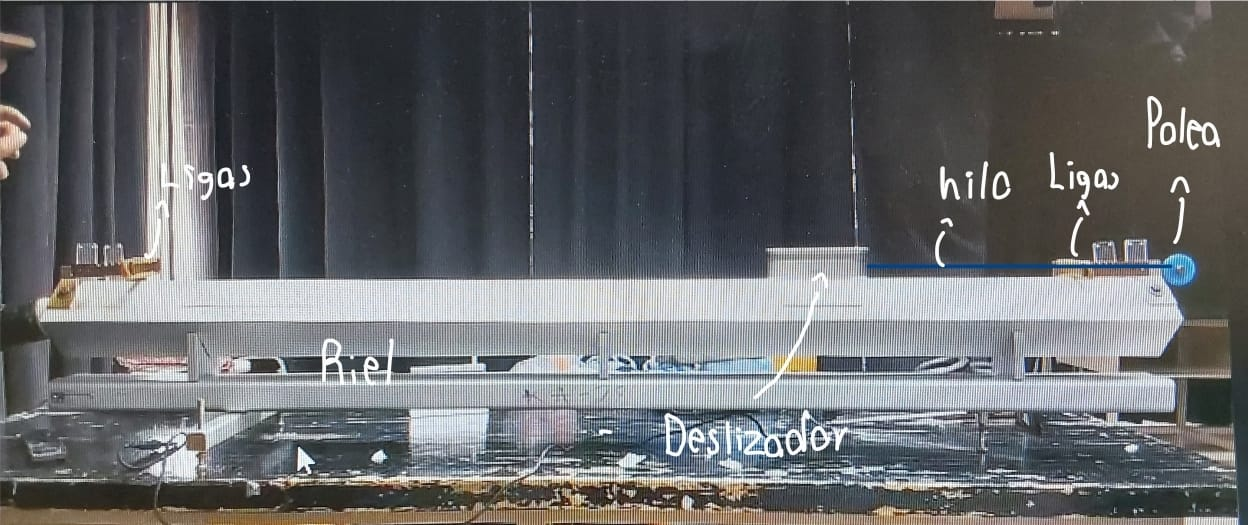
\includegraphics[width=0.40\textwidth]{armado de practica 9.jpg}
\caption{ Armado del sistema experimental}
\end{figure}
Coloque el riel de aire en una superficie plana y nivelada para minimizar las interferencias por inclinación.
Asegúrese de que el riel esté limpio y libre de polvo para reducir la fricción.
Coloque el deslizador sobre el riel de aire.
Fije una polea en un extremo del riel, asegurándose de que la polea esté bien alineada y gire libremente sin fricción adicional.
Ate un extremo del hilo al deslizador y pase el hilo por la polea.
Ate el otro extremo del hilo a una pesa calibrada.

Utilice la balanza para medir y registrar la masa del deslizador y las pesas utilizadas.
Verifique que el hilo esté tenso pero no demasiado, para evitar oscilaciones que puedan afectar las mediciones.

Coloque el deslizador en una posición inicial fija en el riel.
Asegúrese de que el deslizador esté quieto antes de soltar la pesa para garantizar que la velocidad inicial sea cero.
Verifique que el riel de aire esté encendido y funcionando correctamente, proporcionando una superficie de baja fricción.

Suelte la pesa y permita que el deslizador se mueva a lo largo del riel.
Utilice el cronómetro digital o los sensores de velocidad para medir la velocidad del deslizador en diferentes puntos de su recorrido.

\hfill 

\section{RESULTADOS}

La velocidad obtenida mediante recursos audiovisuales se muestra en la tabla 1 para diferentes pruebas.
\begin{table}[!ht]
    \centering
     \caption{\ Periodo del péndulo de longitud 1 metro, comparación del cronómetro y el sensor.}
    \begin{tabular}{|l|l|}
    \hline
        Sensor & Cronómetro \\ \hline
        Número de lanzamiento & velocidad ± 0.05m/s \\ \hline
        
        Lanzamiento 1 & 0. 815 \\ \hline
        Lanzamiento 2 & 1.024 \\ \hline
        Lanzamiento 3 & 1.064\\ \hline
    \end{tabular}
\end{table}\\

De los datos se obuvo en en promedio la velocidad en este punto fue de (0.968 ± 0.134) m/s

Con base a la toría sobre el teorema trabajo-energía calculamos la energía cinética :
\begin{equation}\label{eq:6}
    k_f = \frac{1}{2}(m_1+m_2)v^2
\end{equation}
Donde  m1 y m2 son las masas del riel y la pesa respectivamente; y v es la velocidad obtenida experimentalmente.
Sustituyendo se llega a un valor de \(k_f = 0.145J \pm 0.153\).
Por otra parte, el resultado teórico que predice el modelo es 0.2207J



\section{DISCUSIÓN}
Los resultados experimentales obtenidos muestran que la energía cinética del deslizador es de \(k_f = 0.145J \pm 0.153\).
 Comparando este valor con el resultado teórico de 
0.2207
Joules observamos una discrepancia significativa.

La hipótesis planteada establecía que el trabajo neto realizado sobre el deslizador por la fuerza aplicada sería igual al cambio en su energía cinética. Dado que el resultado experimental de la energía cinética difiere notablemente del valor teórico 
 la hipótesis no puede ser confirmada con los datos actuales. La discrepancia entre los valores sugiere que hay factores adicionales que afectaron los resultados experimentales.

El teorema del trabajo y la energía establece que el trabajo neto realizado sobre un objeto es igual a su cambio en energía cinética. En un sistema ideal, sin pérdidas por fricción u otros factores externos, los valores experimentales deberían coincidir estrechamente con los teóricos. En este caso, la diferencia entre los resultados indica que el sistema experimental no se comportó de manera completamente ideal.

Las posibles razones para las discrepancias observadas pueden incluir: Fricción Residual, Alineación y Tensado del Hilo, Precisión de las Mediciones, Pérdidas de Energía.

Para mejorar la precisión de futuros experimentos y reducir las discrepancias, se podrían implementar las siguientes mejoras:
Optimización del Sistema de Riel de Aire: Asegurar un mantenimiento regular del riel de aire y verificar su calibración antes de cada experimento.
Mejora de la Alineación y Tensado: Utilizar dispositivos de alineación más precisos y sistemas de tensado controlado para el hilo.
Repetición y Promediado: Realizar un mayor número de repeticiones del experimento para obtener un conjunto de datos más robusto y reducir el impacto de errores aleatorios.

\section{ CONCLUSIONES} 
En esta práctica de laboratorio, se investigó la relación entre el trabajo y la energía cinética de un deslizador en un riel de aire. Aunque los resultados experimentales 

\begin{equation}\label{eq:6}
    k_f = (0.145 \pm 0.153)J
\end{equation}

se identificaron factores como la fricción residual y la precisión de las mediciones que pueden haber afectado los resultados. Los objetivos de medir y analizar el trabajo y la energía cinética se lograron, proporcionando una comprensión más profunda de estos conceptos y destacando áreas de mejora para futuros experimentos.



% you can choose not to have a title for an appendix
% if you want by leaving the argument blank
\section{ REFERENCIAS}
\begin{itemize}
\item Serway, R. A., Jewett, J. W. (2008). "Física para ciencias e ingeniería.".
\item Resnick-Halliday. "Física Vol. 2, 5$^{ta}$ Edición, Editorial CECSA, México, 2005".
\item Aranzeta, C. G. (1986). "Introducción a la metodología experimental."
\item Oda-Noda, B. (2005). "Introducción al análisis gráfico de datos experimentales." 
\end{itemize}
% use section* for acknowledgment







\end{document}